\documentclass{beamer}
\usepackage{subfig}
\usepackage{amsmath}
\usepackage{bm}


\DeclareMathOperator*{\argmax}{arg\,max}
\DeclareMathOperator*{\argmin}{arg\,min}

\setbeamertemplate{footline}[frame number]
\title{Linear Regression}
\author{Prof. Alessandro Lucantonio}
\institute{Aarhus University}
\date{7/10/2024}

\setbeamertemplate{navigation symbols}{}


\begin{document}
	
	\frame{\titlepage}
	
	\section{Linear regression with one variable}

	\begin{frame}
		\frametitle{Weight-Height dataset}
		
		Task: build a model that predicts the height given the weight. 
		
		\begin{figure}
			\centering
			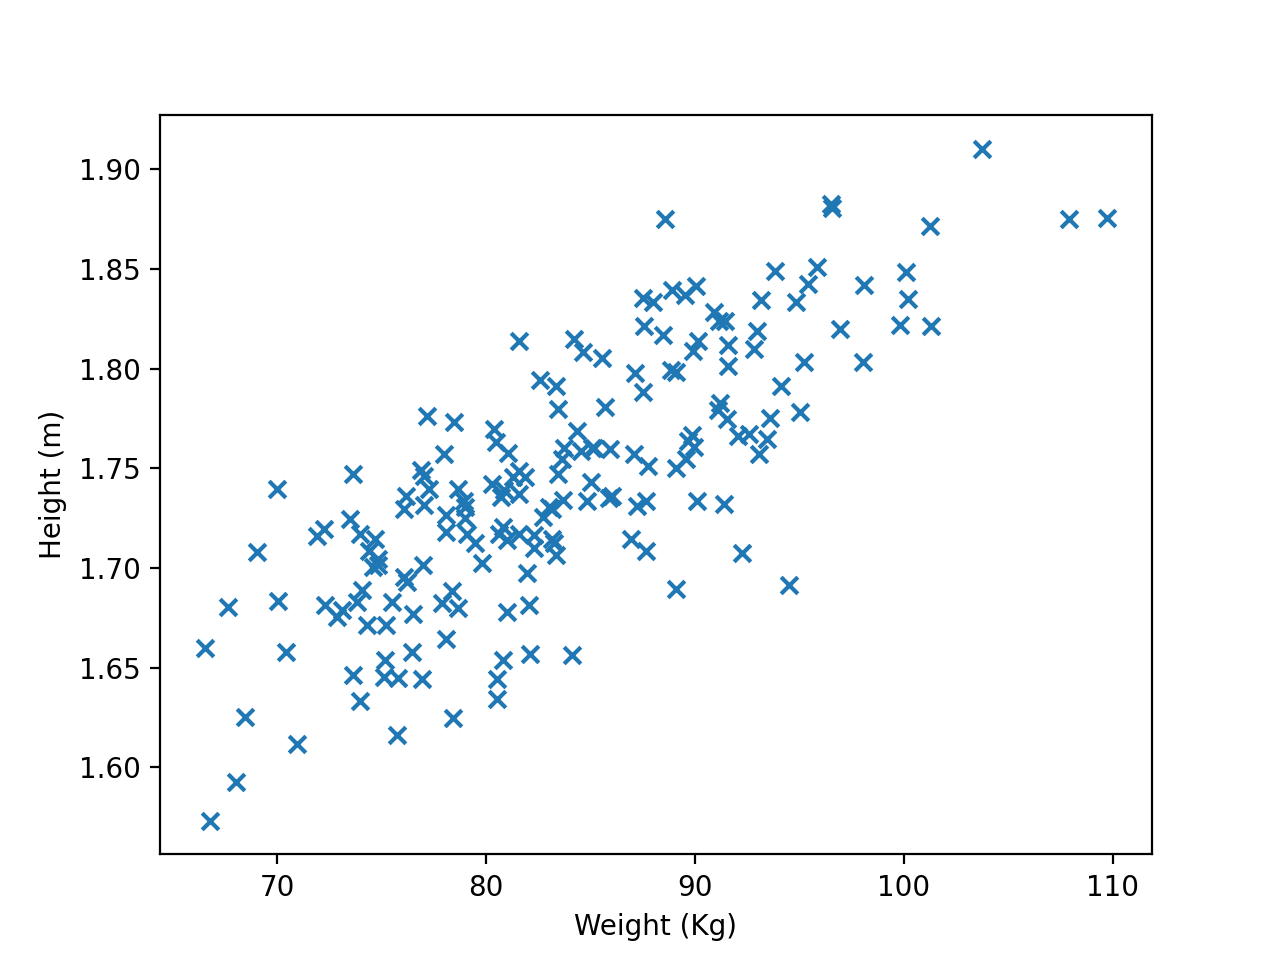
\includegraphics[scale=0.5]{images/linear_regression_data}
			\caption{Plot of the dataset}
		\end{figure}
	\end{frame}

	\begin{frame}
		\frametitle{A solution - Linear Regression model}
		Remarks:
		\begin{itemize}
			\item Regression problem (continuous output).
			\item Data with different orders of magnitude.
		\end{itemize}
		A possible solution to this problem is a linear model (red line in the figure below). This learning algorithm is called \textbf{Linear Regression} (LR).
		\vspace{-5mm}
		\begin{figure}
			\centering
			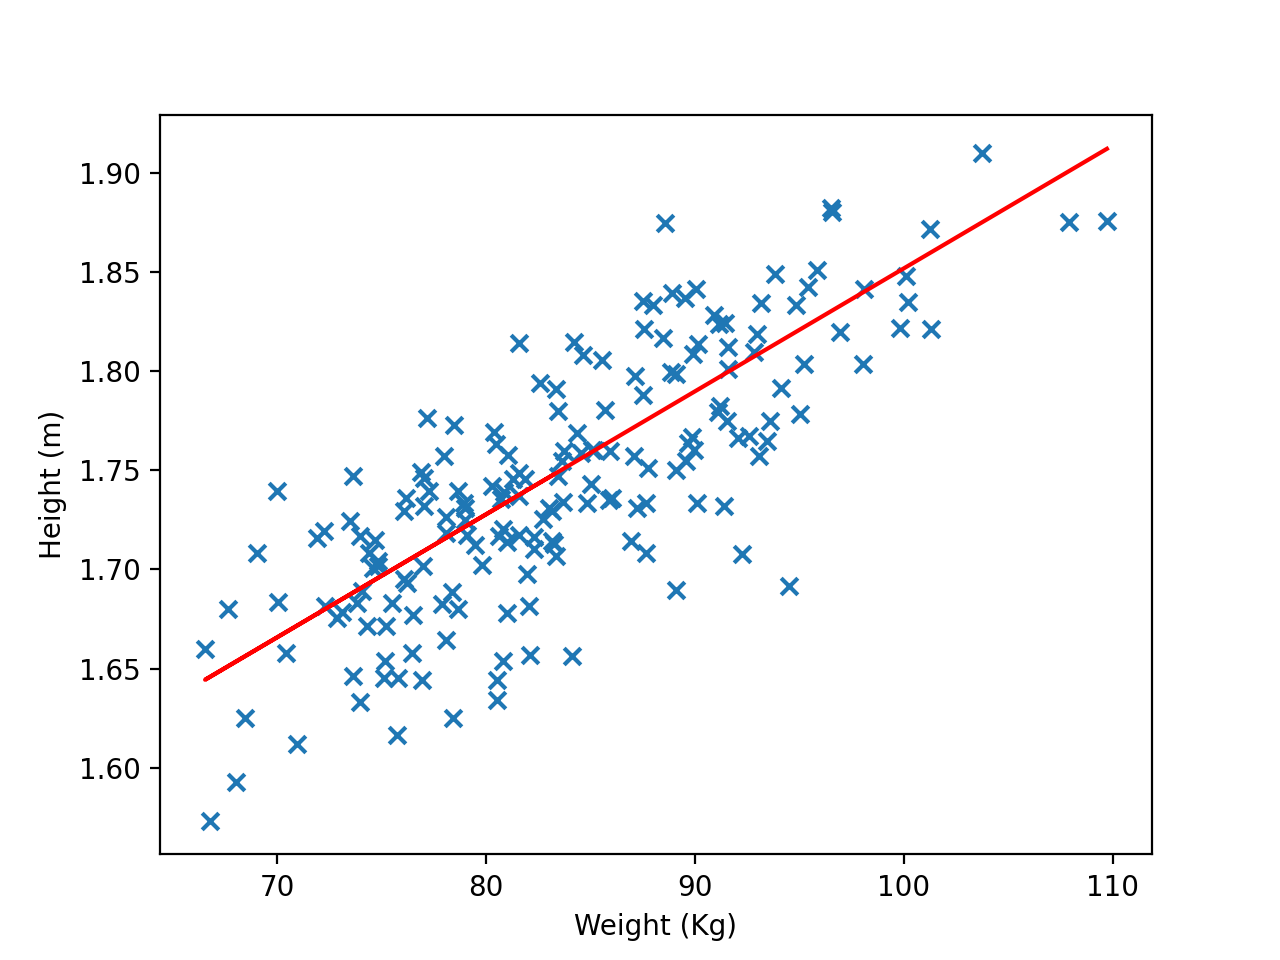
\includegraphics[scale=0.4]{images/linear_regression_fit}
			\caption{Linear regression model.}
		\end{figure}
	\end{frame}

	\begin{frame}
		\frametitle{Linear Regression: main ingredients}
		Notation:
		\begin{itemize}
			\item $x^{(i)}$: a data sample (weight of the $i$-th person).
			\item $y^{(i)}$: the target corresponding to $x^{(i)}$ (height).
			\item $N$: number of samples.
		\end{itemize}
	
		\vspace{5 mm}
		
		\textbf{Model/hypothesis}: 
		\begin{align*}
			h_{\bm{w}}(x^{(i)}) = w_1x^{(i)} + w_0
		\end{align*}
		where $\bm{w} = [w_0, w_1]^T$ is the vector of parameters to be learned.
		
		\vspace{5 mm}
		
		The set $\mathcal{H}:= \{h_{\bm{w}}| \bm{w} \in \mathbb{R}^2\}$ is called \textbf{hypothesis space}.
		
		\vspace{5 mm}
		
		How to learn $\bm{w}$ from data?
		
	\end{frame}



	\begin{frame}
		\frametitle{Performance measure: Mean Squared Error (MSE)}
		\begin{itemize}
			\item As a loss function (performance measure) for the LR problem, we use the \textbf{Mean Squared Error} (MSE):
			$$E({\bm{w}}) := \frac{1}{N} \sum_{i=1}^{N} (h_{\bm{w}}(x^{(i)}) - y^{(i)})^2.$$
			\item To find the ``best" set of parameters, we minimize the loss:
			
			$$\bm{w} \in \argmin_{\bm{\theta} \in \mathbb{R}^2} E(\bm{\theta}).$$
		\end{itemize}
	\end{frame}

	\begin{frame}
		\frametitle{MSE - Visualization}
		\begin{figure}
			\centering
			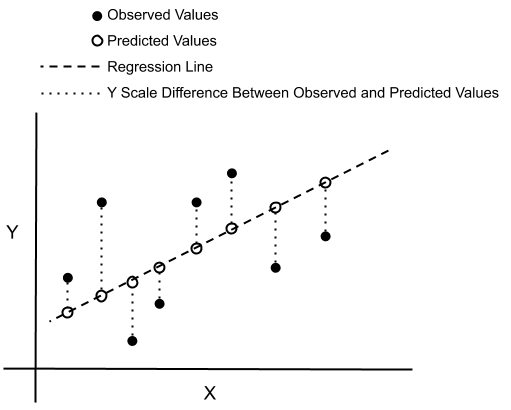
\includegraphics[scale=0.5]{images/mse}
		\end{figure}
	\end{frame}
	
	\begin{frame}
		\frametitle{Digression: Maximum Likelihood Estimation}
		\begin{itemize}
			\item $p_{\rm data}(x)$: data-generating distribution (unknown)
			\item $p_{\rm model}(x; \bm{\theta})$: mapping of each configuration $x$ into a real number estimating the true probability $p_{\rm data}(x)$, for a given set of parameters $\bm{\theta}$
		\end{itemize}	
		\vspace{2mm}
		\textit{Maximum Likelihood Estimator}:
		$$ \bm{w} = \argmax_{\bm{\theta}} \prod_{i=1}^{N} p_{\rm model}(x^{(i)}; \bm{\theta}) $$
		Take the log (does not change argmax) and divide by $N$:
		\begin{align*}
			\bm{w} &= \argmax_{\bm{\theta}}\mathbb{E}_{x \sim \hat{p}_{\rm data}} [\log p_{\rm model}(x; \bm{\theta})] \\
			&= -\argmin_{\bm{\theta}}\mathbb{E}_{x \sim \hat{p}_{\rm data}} [\log p_{\rm model}(x; \bm{\theta})]
		\end{align*} 
		where $\hat{p}_{\rm data}$ is the \textbf{empirical distribution} defined by the training data.
		This is equivalent to minimizing the \textit{dissimilarity} (or \textit{cross-entropy}) between $ \hat{p}_{\rm data}$ and $p_{\rm model}$:
		$$ \mathbb{E}_{x \sim \hat{p}_{\rm data}} [\log \hat{p}_{\rm data}(x)-\log p_{\rm model}(x; \bm{\theta})] $$
	\end{frame}
	
	\begin{frame}
		\frametitle{Conditional Log-Likelihood and MSE}
		The MLE estimator can be generalized to estimate a conditional probability $P(y^{(i)} | x^{(i)}; \bm{\theta})$ in order to predict $y^{(i)}$ given $x^{(i)}$. Assuming the samples are iid, we can write
		\begin{align*}
			\bm{w} &= \argmax_{\bm{\theta}}\sum_{i=1}^{N}\log P(y^{(i)} | x^{(i)}; \bm{\theta})
		\end{align*} 
		Think of the model as producing a conditional probability distribution. Assume:
		$$ P(y^{(i)} | x^{(i)}; \bm{\theta}) = \frac{1}{\sqrt{2\pi\sigma^2}} \exp\left(-\frac{\|\hat{y}^{(i)}-y^{(i)}\|^2}{2\sigma^2}\right)$$
		where $\hat{y}^{(i)}$ is the prediction of the mean of the Gaussian. Then
		$$\sum_{i=1}^{N}\log P(y^{(i)} | x^{(i)}; \bm{\theta}) = -N\log \sigma - \frac{N}{2}\log (2\pi) - \sum_{i=1}^{N}\frac{\|\hat{y}^{(i)}-y^{(i)}\|^2}{2\sigma^2}$$
	\end{frame}
	
	\begin{frame}
		\frametitle{Conditional Log-Likelihood and MSE}
		Compare the log-likelihood with MSE:
		$$\sum_{i=1}^{N}\log P(y^{(i)} | x^{(i)}; \bm{\theta}) = -N\log \sigma - \frac{N}{2}\log (2\pi) - \sum_{i=1}^{N}\frac{\|\hat{y}^{(i)}-y^{(i)}\|^2}{2\sigma^2}$$
		$$ \textrm{MSE} = \frac{1}{N}  \sum_{i=1}^{N}\|\hat{y}^{(i)}-y^{(i)}\|^2$$
		\textit{Maximizing} the \textbf{log-likelihood }with respect to the parameters yields the same estimate of them as does \textit{minimizing} the \textbf{MSE}.
		
	\end{frame}

	\begin{frame}
		\frametitle{Multiple-feature Linear Regression}
		
		\begin{itemize}
			\item Dataset: $\bm{x}^{(i)} \in \mathbb{R}^n, y^{(i)} \in \mathbb{R}$, where
			$x^{(i)}_j$ is the $j$-th feature of the $i$-th sample and $n$ is the number of features.
			\item Hypothesis: 
			\begin{align*}
				h_{\bm{w}}(\bm{x}^{(i)}) &= w_{n}x^{(i)}_n + w_{n-1}x^{(i)}_{n-1} + \dots + w_1 x^{(i)}_1 + w_0\\
				&= \sum_{j=0}^n w_j \tilde{x}^{(i)}_j = \mathsf{X}\bm{w},
			\end{align*}
			where
				\begin{equation*}
				\mathsf{X} = \begin{bmatrix}
					\tilde{\bm{x}}^{(1)}\\
					\vdots\\
					\tilde{\bm{x}}^{(N)}
				\end{bmatrix} \in \mathbb{R}^{N \times (n+1)}
			\end{equation*}
			with $\tilde{\bm{x}}^{(i)} = [1, x^{(i)}_1, \dots, x^{(i)}_n]$ and $\bm{w} = [w_0, \dots, w_n]^T$.
		\end{itemize}
		
	\end{frame}

	\begin{frame}
		\frametitle{Multiple-feature Linear Regression - MSE}
		The MSE can be computed using matrix-vector operations:
		\begin{align*}
			E(\bm{w}) &= \frac{1}{N} \sum_{i=1}^{N} (h_{\bm{w}}(\bm{x}^{(i)}) - y^{(i)})^2 = \frac{1}{N} (\mathsf{X} \bm{w} - \bm{y})^T (\mathsf{X}\bm{w} - \bm{y})\\
			&= \frac{1}{N} ||\mathsf{X}\bm{w} - \bm{y}||^2,
		\end{align*}
		where
		\begin{equation*}
			 \bm{y} = \begin{bmatrix}
			y^{(1)} \\
			\vdots\\
			y^{(N)}
		\end{bmatrix} \in \mathbb{R}^N.
		\end{equation*}
	\end{frame}

	\begin{frame}
		\frametitle{Coefficient of determination}		
		
		The coefficient of determination (usually denoted by $R^2$) is a statistical measure that can be used to evaluate the goodness of fit of a regression model. It is defined as:
		\begin{equation*}
			R^2 := 1 - \frac{||\bm{\epsilon}||^2}{\sigma_{\bm{y}}^2}
		\end{equation*}
		where $\bm{\epsilon} := \bm{y} - \mathsf{X}\bm{w}$ is the vector of the \textit{residuals} and $\sigma_{\bm{y}}:= \sqrt{\text{Var}(\bm{y})}$ the standard deviation of the targets. 
		
		\vspace{5mm}
		
		Perfect fit: $\sigma_{\bm{\epsilon}} = 0$, hence $R^2 = 1$. Notice: $R^2$ \textit{may} be negative.
		
	\end{frame}

	\begin{frame}
		\frametitle{Finding the minimum: Gradient Descent}
		How to find the optimal weights $\bm{w}$?
		
		\vspace{5mm}
		
		Main idea: geometrically, the gradient of a scalar function points in the direction of maximum growth. Hence, following the direction opposite to the gradient allows to decrease the value of the function, \textit{i.e.}
		\begin{equation*}
			E(\bm{w}^{j+1}) \leq E(\bm{w}^j) 
		\end{equation*}
		
		\vspace{5mm}
		
		Formally:
		\begin{itemize}
			\item Start with an initial guess $\bm{w}^0$.
			\item For $j \geq 0$, update $\bm{w}^{j+1} := \bm{w}^{j} + \bm{d}^j$, where $\bm{d}^j$ is such that
			$$\bm{d}^j = - \alpha \nabla E(\bm{w}^j)$$
			where $\alpha>0$ is the \textbf{learning rate}.
		\end{itemize}
	
	\end{frame}

	\begin{frame}
		\frametitle{Gradient Descent - 3D visualization}
		\begin{figure}
			\centering
			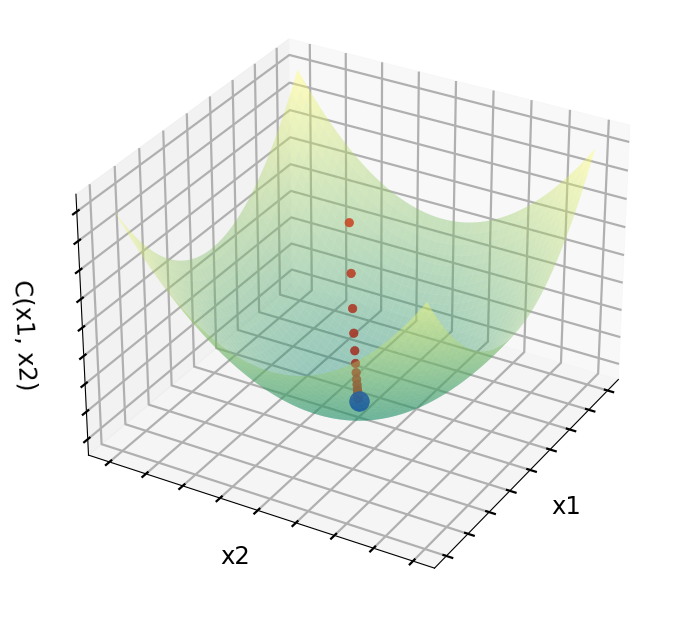
\includegraphics[scale=0.4]{images/gradient_descent_3D}
			\caption{In blue, the global minimum, in red, the iteration points.}
		\end{figure}
	\end{frame}

	\begin{frame}
		\frametitle{Gradient Descent: Effect of the learning rate/1}
		\begin{figure}
			\centering
			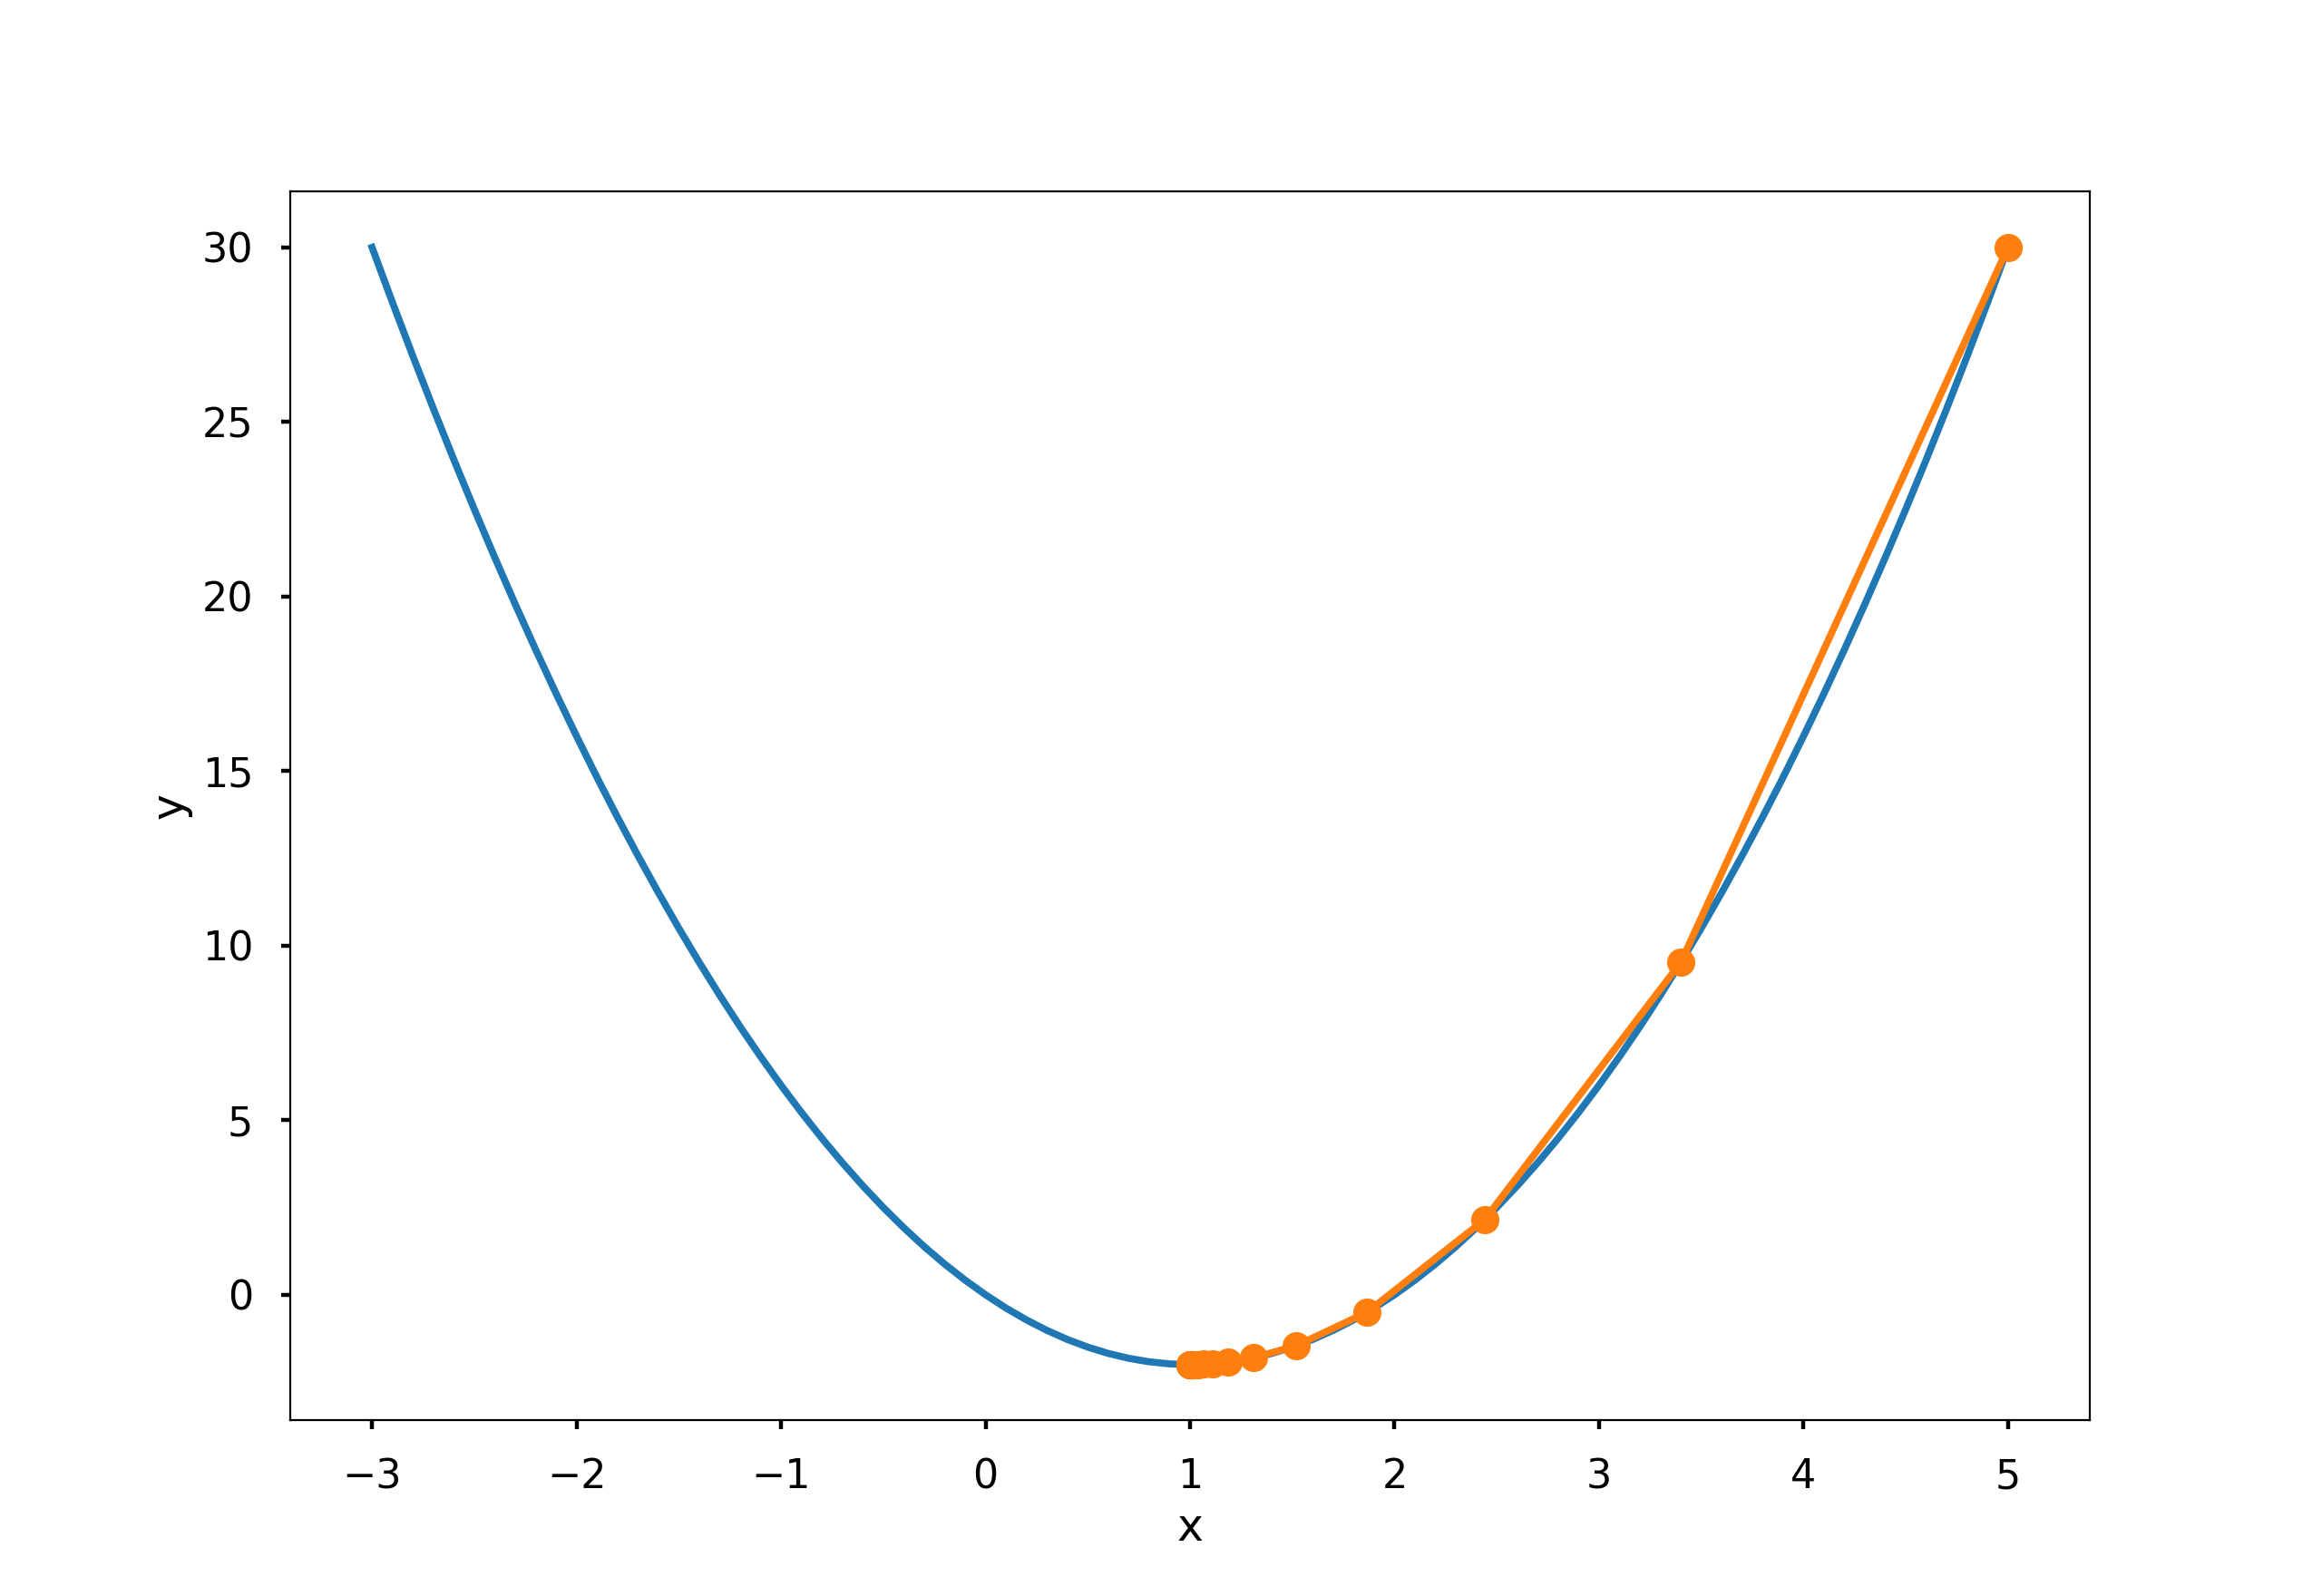
\includegraphics[scale=0.3]{images/gradient_descent_1}
			\caption{Learning rate = 0.1.}
		\end{figure}
	\end{frame}

	\begin{frame}
		\frametitle{Gradient Descent: Effect of the learning rate/2}
		\begin{figure}
			\centering
			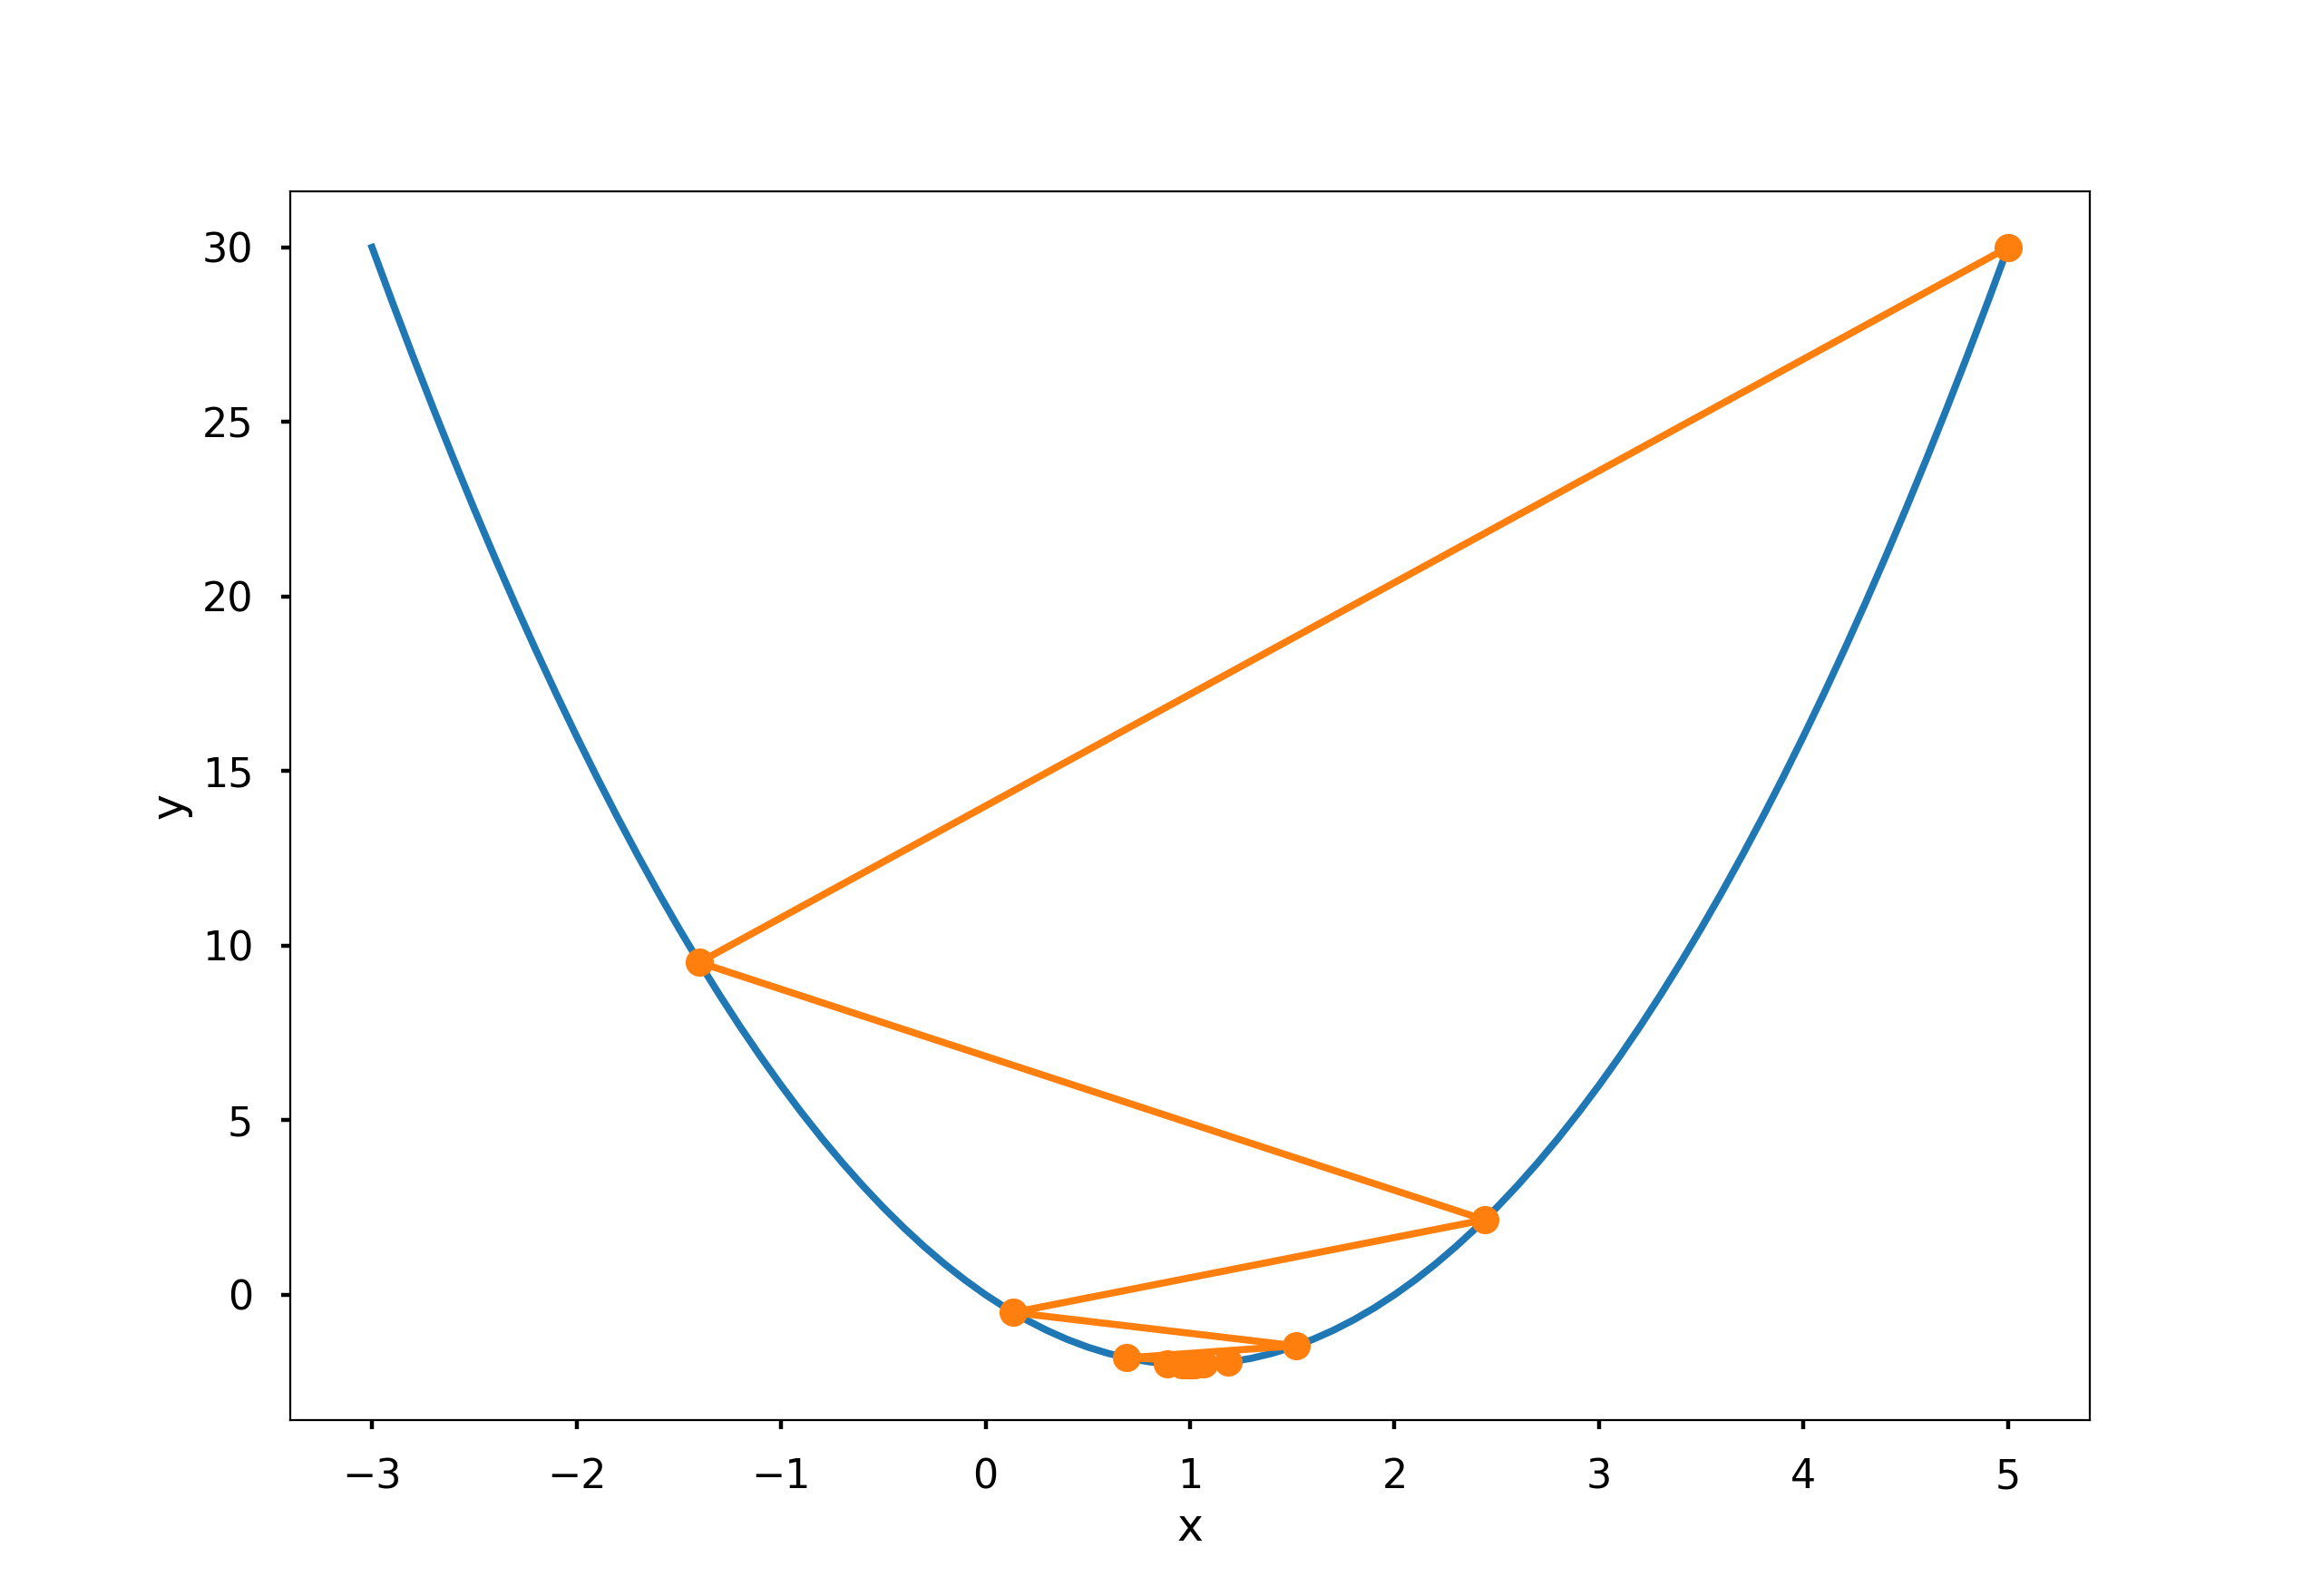
\includegraphics[scale=0.3]{images/gradient_descent_2}
			\caption{Learning rate = 0.4.}
		\end{figure}
	\end{frame}

	\begin{frame}
		\frametitle{Gradient Descent: Effect of the learning rate/3}
		\begin{figure}
			\centering
			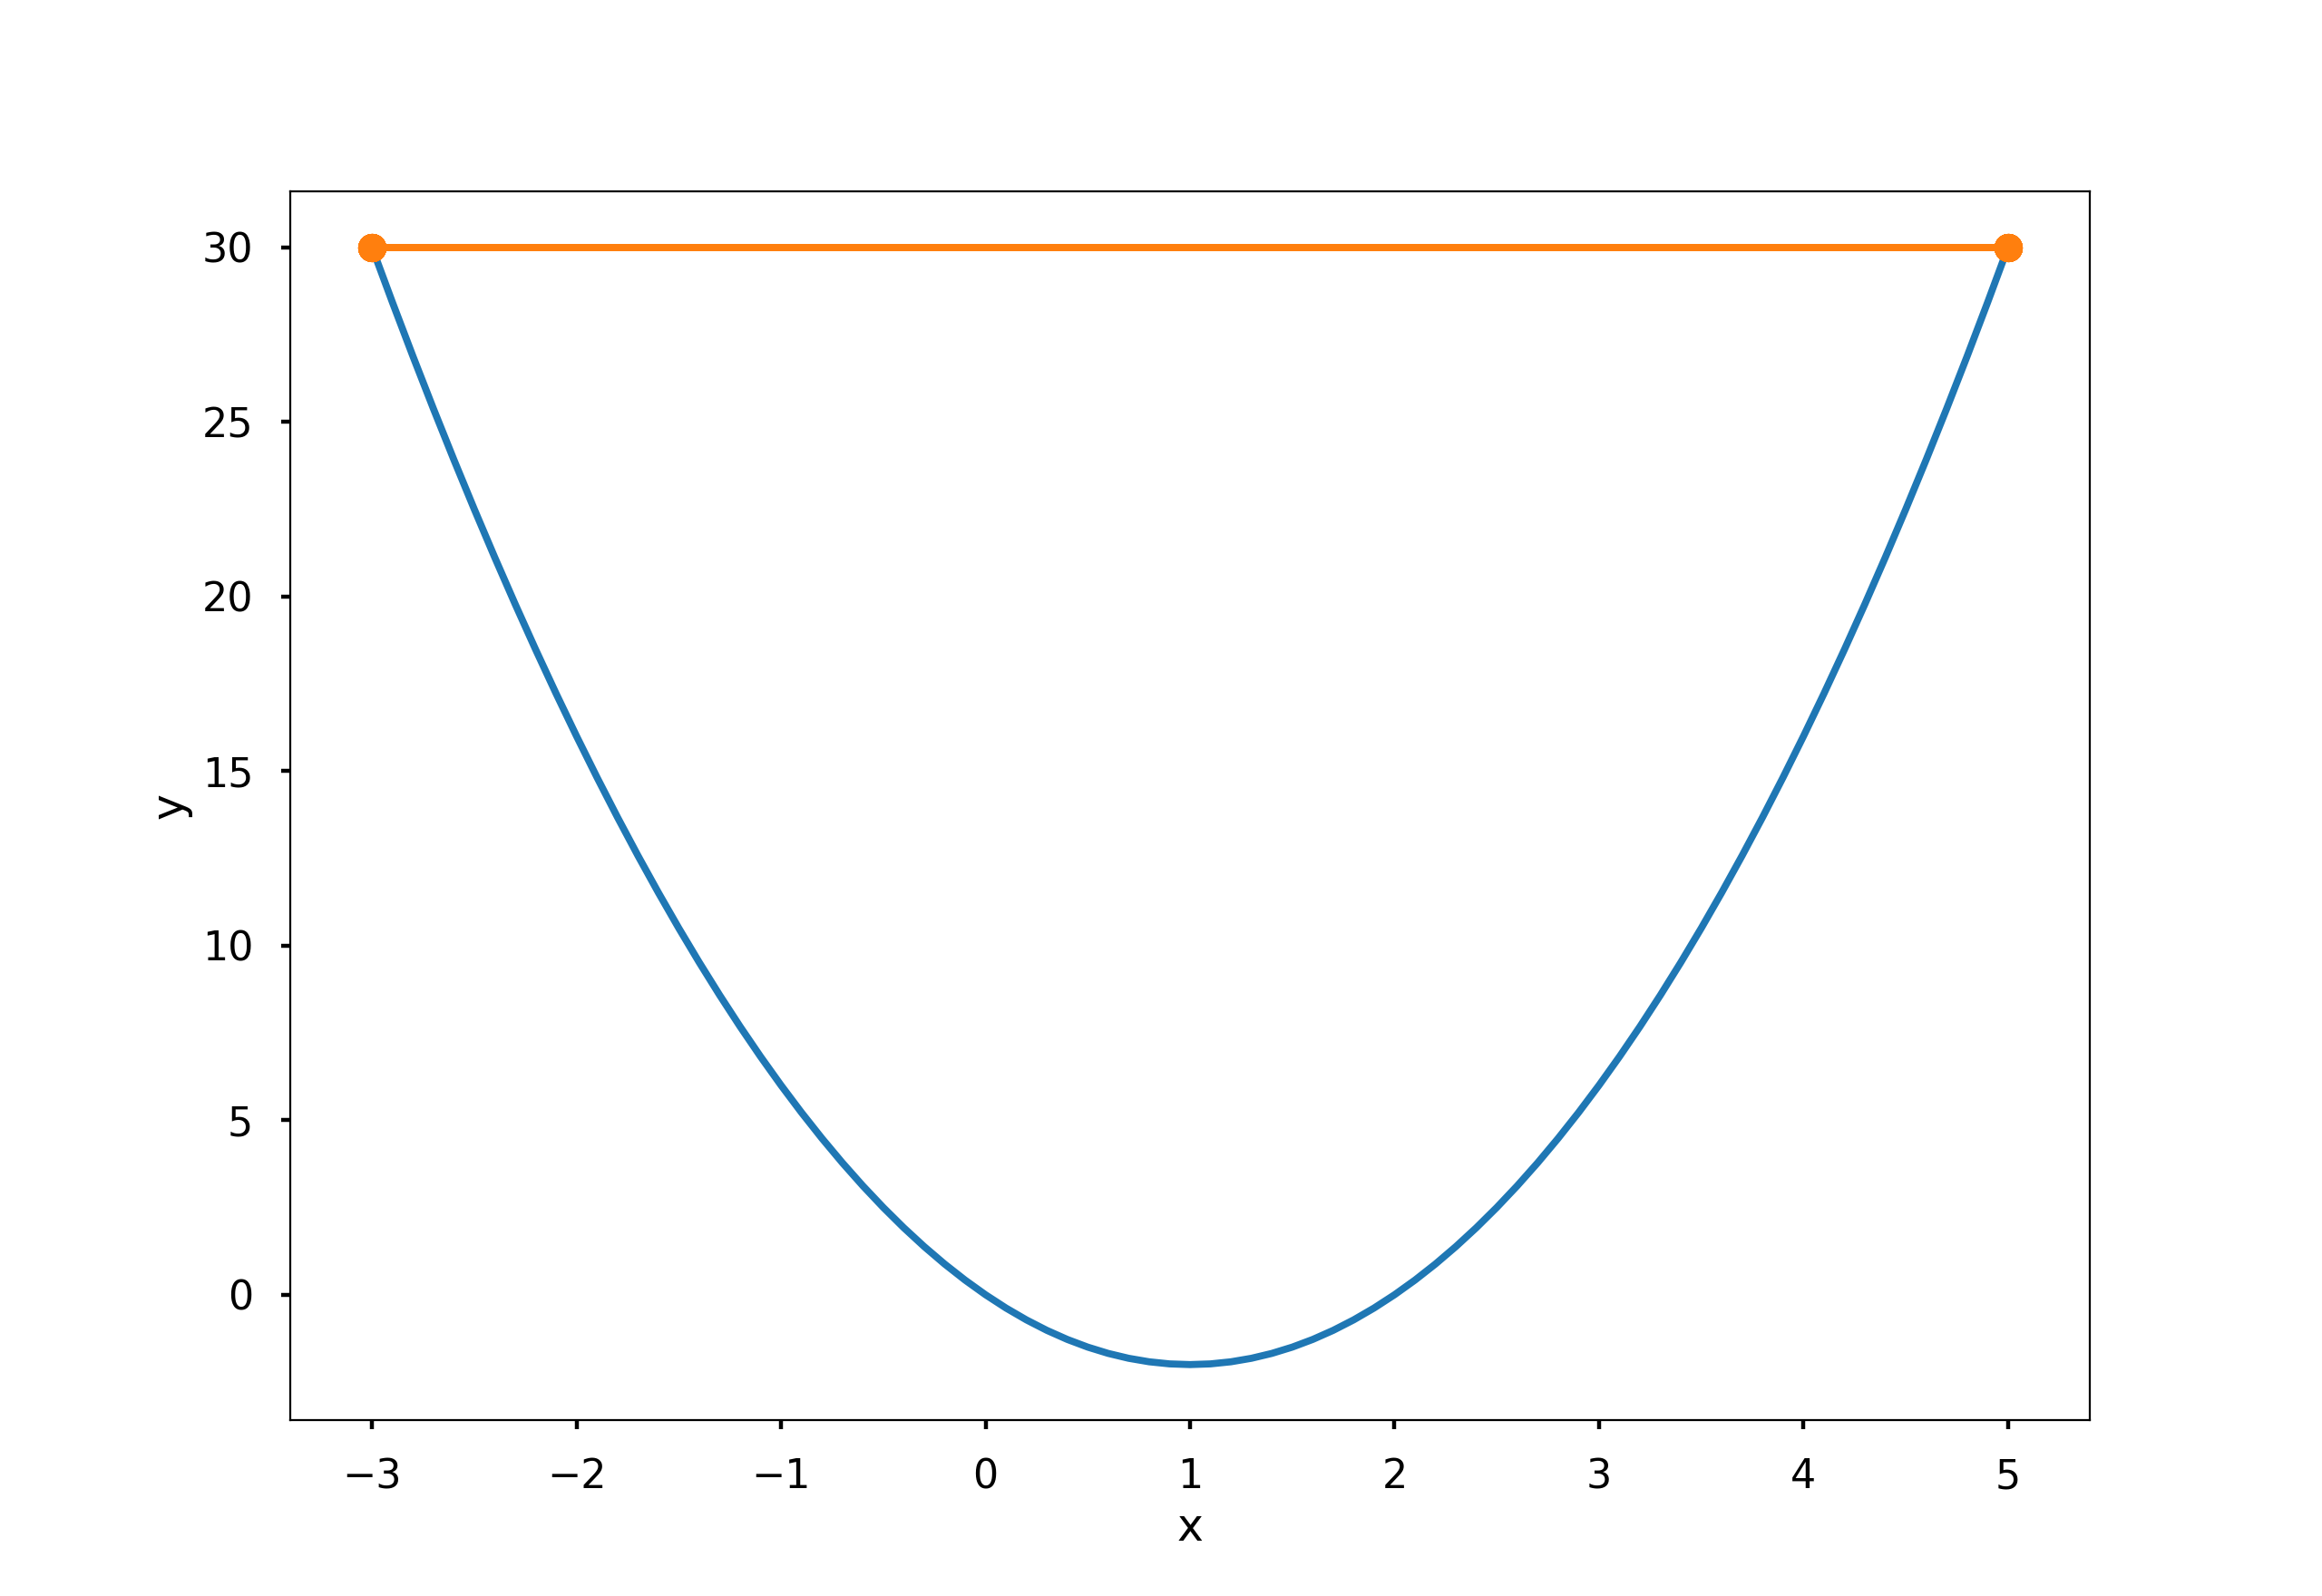
\includegraphics[scale=0.3]{images/gradient_descent_3}
			\caption{Learning rate = 0.5.}
		\end{figure}
	\end{frame}

	\begin{frame}
		\frametitle{Batch GD, SGD and Mini-Batch GD - Intuition}
		
		For a dataset consisting of multiple samples, the loss function can be computed by summing over samples:
		
		$$E(\bm{w}) = \frac{1}{N} \sum_{i=1}^N E_i(\bm{w})$$
		
		\begin{itemize}
			\item The classical gradient descent update rule, \textit{i.e.} update the weights based on the gradient of the entire cost $E(\bm{w})$, is called \textbf{batch version}. However, for large $N$ computing $\nabla E(\bm{w})$ is very time consuming.
			
			\item To speed-up the update rule we approximate $\nabla E(\bm{w})$ with $\nabla E_i(\bm{w})$. This is the idea behind the so-called \textbf{Stochastic Gradient Descent} (SGD) or \textbf{online version}.
			
			\item A trade-off between batch GD and SGD is called the \textbf{mini-batch} GD.
		\end{itemize}
		
	\end{frame}

	\begin{frame}
		\frametitle{Batch GD, SGD and Mini-Batch GD - Algorithms}
		
		
		\textbf{Batch GD}:
		\begin{itemize}
			\item Start with an initial guess $\bm{w}^0$.
			\item For $j \geq 0$, update $\bm{w}^{j+1} = \bm{w}^{j} - \alpha \nabla E(\bm{w}^j)$.
		\end{itemize}
		
		\textbf{SGD} (online):
		\begin{itemize}
			\item Start with an initial guess $\bm{w}^0$.
			\item For each epoch $j \geq 0$:
			\begin{itemize}
				\item draw a random sample $i$ from the dataset;
				\item for each $1\leq i \leq N$ update $\bm{w}^{j+1} = \bm{w}^j - \alpha \nabla E_i(\bm{w}^j)$.
			\end{itemize}
		\end{itemize}
	
		\textbf{Mini-Batch GD}:
		\begin{itemize}
			\item Fix an integer $1 \leq \text{mb} \leq N$ (mini-batch size).
			\item Start with an initial guess $\bm{w}^0$.
			\item For each epoch $j \geq 0$:
			\begin{itemize}
				\item draw a random batch from the dataset;
				\item for each $0 \leq i < \frac{N}{\text{mb}}$ update
				\begin{equation*}
					\bm{w}^{j+1} = \bm{w}^j - \alpha \nabla \sum_{k=i\cdot\text{mb} + 1}^{(i+1)\cdot\text{mb}}E_k(\bm{w}^j).
				\end{equation*}
			\end{itemize} 
		\end{itemize}
		
	\end{frame}

	\begin{frame}
		\frametitle{How to choose among different variants?}
		\begin{itemize}
			\item Batch: usually more stable and provide a more accurate estimation of the gradient, but slow.
			\item SGD: fast, stochastic approximation of the gradient implies possible instability (zig-zag effect)
			\item Mini-Batch GD: a trade-off between Batch GD and SGD (parallelism available).
		\end{itemize}
	%In practice, through SGD and Mini-Batch GD we may not even reach the minimum, but it is enough to get close to it.
		\begin{figure}
			\centering
			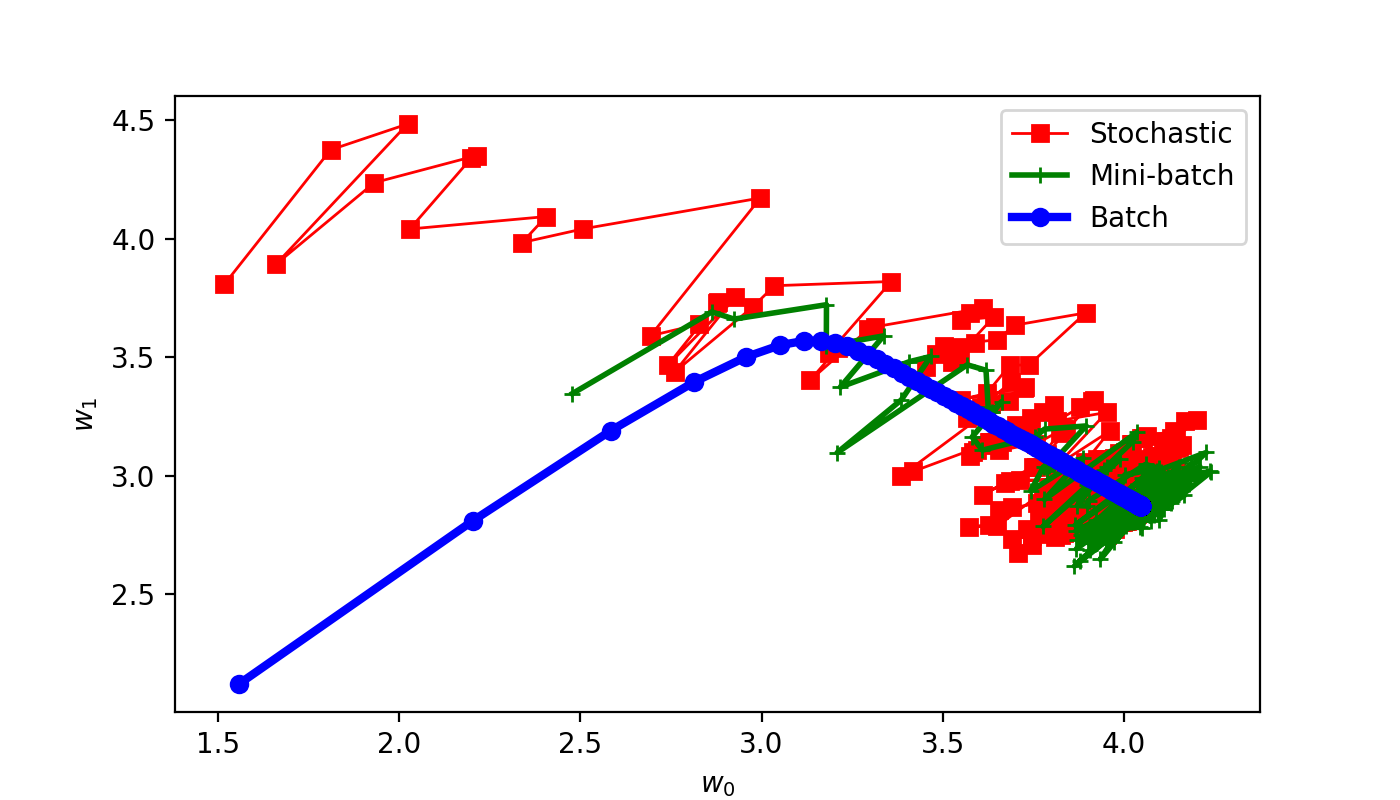
\includegraphics[scale=0.42]{images/gd_mb_sgd}
			\caption{Batch GD vs SGD vs Mini-Batch GD.}
		\end{figure}
	
	\end{frame}

	\begin{frame}
		\frametitle{Normal Equation for LR and Gradient Descent}
		We have $E(\bm{w}) = \frac{1}{N} ||\mathsf{X}\bm{w} - \bm{y}||^2$, hence
		\begin{equation*}
			\nabla E(\bm{w}) = \frac{1}{N} \nabla (||\mathsf{X}\bm{w} - \bm{y}||^2) = \frac{2}{N}\mathsf{X}^T(\mathsf{X}\bm{w} - \bm{y})
		\end{equation*}
	
	\begin{itemize}
		\item 	Normal equation ($\textcolor{red}{\iff}$ holds if $\mathsf{X}^T\mathsf{X}$ is invertible):
		\begin{align*}
			\nabla E(\bm{w}) = 0 &\iff \frac{2}{N}\mathsf{X}^T(\mathsf{X}\bm{w} - \bm{y}) = 0\\ 
			&\iff \mathsf{X}^T\mathsf{X}\bm{w} = \mathsf{X}^T\bm{y}\\
			& \textcolor{red}{\iff} \bm{w} = (\mathsf{X}^T\mathsf{X})^{-1}\mathsf{X}^T\bm{y}
		\end{align*}
		\item Gradient descent main iteration for LR:
		\begin{equation*}
			\bm{w}^{j+1} = \bm{w}^{j} - \frac{2\alpha}{N}\mathsf{X}^T(\mathsf{X}\bm{w}^j - \bm{y})
		\end{equation*}
	\end{itemize}

	\end{frame}

	\begin{frame}
		\frametitle{On the invertibility of $\mathsf{X}^T\mathsf{X}$}
		
		Invertibility of $\mathsf{X}^T\mathsf{X} \iff$ columns of $X$ linearly independent.
		
		\vspace{5mm}
		
		What if $\mathsf{X}^T\mathsf{X}$ is not invertible?
		
		\vspace{5mm}
		
		If two columns are linearly dependent, then those features are correlated (\textbf{redundant}).
		
		\vspace{5mm}
		
		Solution: discard one of those features.
	\end{frame}

	\begin{frame}
		\frametitle{Normal Equation vs Gradient Descent}
		Normal equation:
		\begin{itemize}
			\item No hyperparameters (explicit solution).
			\item No iterations.
			\item Computational cost dominated by inversion of a dense matrix (slow when $N$ is large).
		\end{itemize}
	
		\vspace{5mm}
	
		Gradient Descent:
		\begin{itemize}
			\item Need to choose the learning rate $\alpha$.
			\item Needs many iterations (usually increase with dataset size).
			\item Cost per iteration lower than matrix inversion (constant when using mini-batch GD), hence faster when $N$ is large.
		\end{itemize}
	\end{frame}


	\begin{frame}
		\frametitle{Dataset scaling}
		In general, features \textbf{must} have similar magnitudes, for good convergence of gradient descent-based methods.
		\vspace{1mm}
		
		\begin{figure}
			\centering
			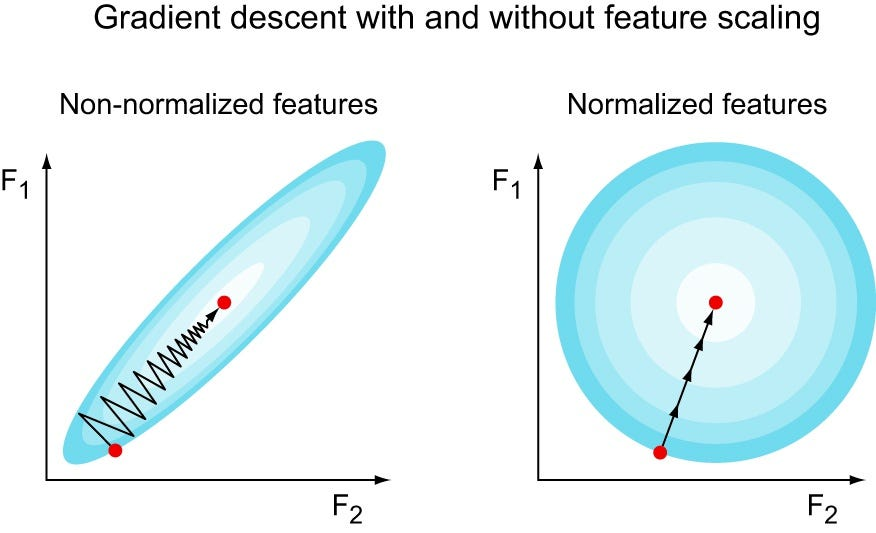
\includegraphics[scale=0.3]{images/feature-scaling}
			\caption{Example loss landscapes with and without feature scaling ($F_1$ and $F_2$ are the weights of the model).}
		\end{figure}
	\end{frame}

	\begin{frame}
		\frametitle{Dataset scaling}
	
		Common approaches:
		\begin{itemize}
			\item \textbf{Min-max scaling}. Compute the feature max $\bm{M} := [\max_i x^{(i)}_j]$ and the feature min $\bm{m} := [\min_i x^{(i)}_j]$ vectors. Then normalize features as follows
			\begin{equation*}
				\bm{x}_{\text{norm}}^{(i)} = \frac{\bm{x}^{(i)} - \bm{m}}{\bm{M} - \bm{m}}
			\end{equation*} 
			\item \textbf{Standardization}. Compute the feature mean $\bm{\mu}$ $(\mu_j := \mathbb{E}_i[x^{(i)}_j])$ and the feature standard deviation $\bm{\sigma}$ $(\sigma_j := \sqrt{\text{Var}_i[x^{(i)}_j]})$. Then normalize features as follows
			\begin{equation*}
				\bm{x}_{\text{norm}}^{(i)} = \frac{\bm{x}^{(i)} -\bm{\mu}}{\bm{\sigma}} 
			\end{equation*}
		\end{itemize}
		
	\end{frame}



	\begin{frame}
		\frametitle{Polynomial Regression}
		Polynomial Regression $\rightarrow$ polynomial hypothesis.
		
		\vspace{5mm}
		
		\textit{Example}: quadratic hypothesis (single feature):	
		
		$$h_{\bm{w}}(x_1) = w_0 + w_1 x_1 + w_2 x_1^2$$
		
		(in case of two features, there is also the term $x_1 x_2$)
		
		\vspace{5mm}
		
		To fit this model, use Linear Regression with features $x_1 = x_1$ and $x_2 = x_1^2$.
	\end{frame}


\end{document}